In this chapter the experiments and the results are presented. In the section of the qualitative results visualizations of the topics are given for different models. It is shown that the topics are meaningful and that semantic descriptions can be given to some of these topics.
In the section of the quantitative results the two developed models are compared with each other and the performance of the model for different number of topics and different number of time-slices are shown.

\section{Qualitative Results}
\subsection{Comparison of the different models}
%wat wordt er in deze sectie getoond?
In this section four different models are compared with each other. The first two models are the LDA model with a Bag-of-word representation, where the dictionary one the one hand is pre-clustered with the k-means algorithm(LDA with BOW + k-means, figure \ref{fig:BOWtopics} a)) and on the other hand not clustered at all (LDA with BOW, figure \ref{fig:BOWtopics} b)). The third and fourth model are LDA-Gaussian and LDA-Poisson (figure \ref{fig:Gaus96} and \ref{fig:Pois96}).\\

% wat is in de plaatjes te zien?
In the following figures the number of time-slices on a day is $N=96$. The time dimension is a coarse-grain representation, which means that there are five different values for the time. The number of topics that are initialized are $k=5$. Figures \ref{fig:BOWtopics} a) + b), \ref{fig:Gaus96} a) and \ref{fig:Pois96} a) are a representation of the topic distribution on different days. There are in total 50 days represented on the y-axis in each figure. On the x-axis the time-slices are shown. The different colors represent the different topics that are assigned to the time-slices.\\

\begin{figure}
 \centering
 \begin{tabular}{c c}
  \centering
  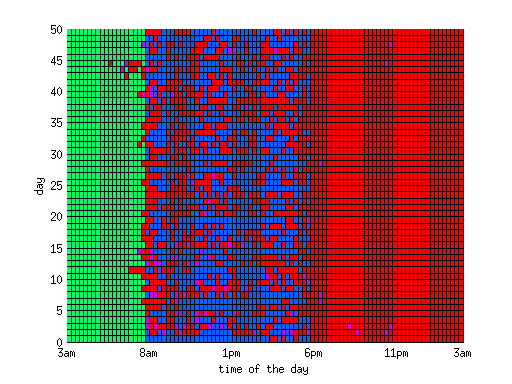
\includegraphics[width=0.45\textwidth]{Pictures/DayTopicsTs96k5Clus.png}
  &
  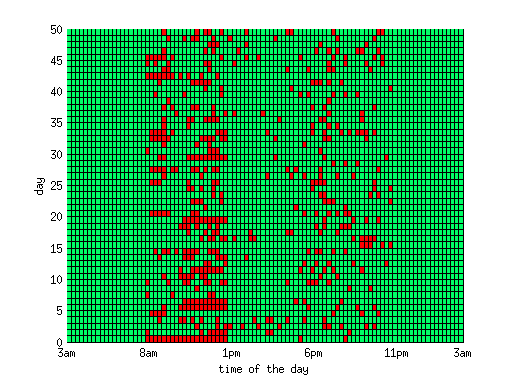
\includegraphics[width=0.45\textwidth]{Pictures/DayTopicsTs96k5bow.png}\\
  a) & b)
 \end{tabular}
 \caption{a) LDA model applied to clustered data. b) LDA applied to data that is not clustered.}
 \label{fig:BOWtopics}
\end{figure}

\pagebreak
 
The LDA model with a BOW-representation is still able to find different topics in the data, although the BOW representation without the clustering only distinguish between two topics (see figure \ref{fig:BOWtopics} b)). If the data is clustered on forehand LDA is able to find four different topics in the data (see figure \ref{fig:BOWtopics} a)). The number of clusters for the k-means algorithms is set to $V=6$. This was the best value to find the most topics in the data. Before the data was clustered, all dimensions where normalized.\\

\begin{figure}
 \centering
 \begin{tabular}{c c}
  \centering
  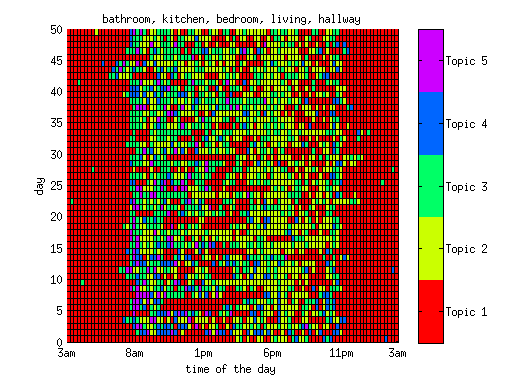
\includegraphics[width=0.45\textwidth]{Pictures/TopDayHN3TS96k5Gaus.png}
  &
  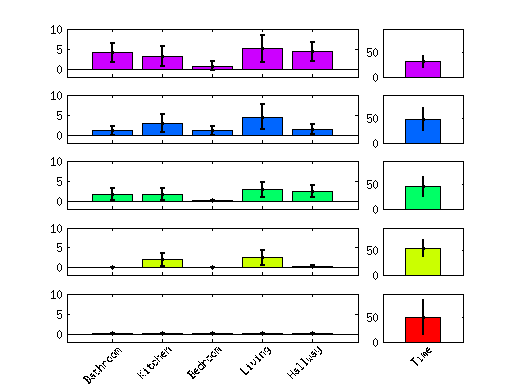
\includegraphics[width=0.45\textwidth]{Pictures/TopVisuHN3TS96k5Gaus.png}\\
    a) & b)
 \end{tabular}
 \caption{Topic distribution per day and the Topic visualization for LDA-Gaussian}
 \label{fig:Gaus96}
\end{figure}  

Figure \ref{fig:Gaus96} shows the outcome of the LDA-Gaussian model. In the figure on the right-hand side (\ref{fig:Gaus96} b) ) the 6 dimensions of the observations are shown on the x-axis. Every topic is marked with a different color and corresponds to the topics in the left image. On the y-axis the mean value $\mu$ of every Gaussian distribution in every dimension is indicated with the height of the bar-chart. The vertical black line represents the standard deviation $\sigma$ of every distribution. The red topic (topic 1) contains a high $\sigma$-value for the time-dimension and captures all time-slice where the value is zero for the sensor values. LDA-Gaussian is able to find more notable topics and leads to more meaningful results than it can found with LDA for a BOW representation. For example the daily structure of a person can be distinguished more easily than it can be done in figure \ref{fig:BOWtopics} a) or b).\\

\pagebreak
\begin{figure}
 \centering
 \begin{tabular}{c c}
  \centering
  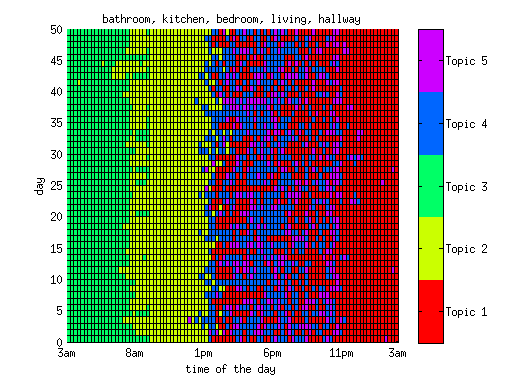
\includegraphics[width=0.45\textwidth]{Pictures/TopDayHN3TS96k5Pois.png}
  &
  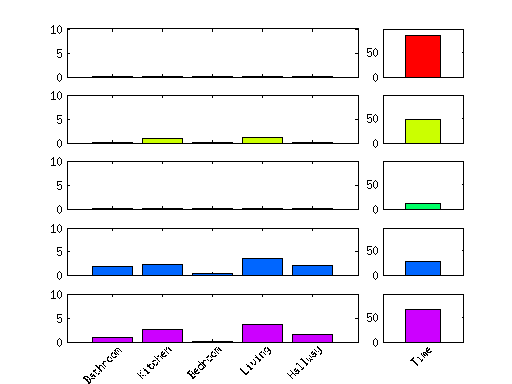
\includegraphics[width=0.45\textwidth]{Pictures/TopVisuHN3TS96k5Pois.png}\\
    a) & b)
 \end{tabular}
 \caption{Topic distribution per day and the Topic visualization for LDA-Poisson}
 \label{fig:Pois96}
\end{figure}  


In figure \ref{fig:Pois96} the outcome of the LDA-Poisson model is shown. The topics that are found are again shown on the right-hand side (\ref{fig:Pois96} b) ). The height of the bars represent the $\lambda$-value of the Poisson-distributions.
In the figure \ref{fig:Pois96} a) five different topics are found. These topics depend however a lot on the time. This is caused by the fact that the Poisson distribution is not a good way to model the time dimension, because small values will have a higher probability in this distribution. Nevertheless LDA-Poisson still performs better, than LDA on the BOW representation.



\subsection{Semantic topic description}
In the following figures the topic distribution for different houses are shown. A semantic description of some topics is given to illustrate the usefulness of the models. The number of time-slices is set to $N=48$. In every figure 50 days are shown. In the left images a) the topic distribution of the days are shown and in the left images b) the topic description for every dimension is given with respectively the same color. For more results see the appendix \ref{chapter:appendix_1}.\\

In figure \ref{fig:HN1Gaus20fine} the outcome for the LDA-Gaussian model is shown. The time dimension has a fine grain representation. The model is initialized with $k=20$ topics and the 10 most important topics are visualized with a different color, the remaining topics have the color gray in the left image. The first topic (red) is an easy topic to find. In all time-slices that are marked with red no activations of the sensors are captured. The time dimension has a big standard deviation, because this topic can occur all day long. In figure \ref{fig:HN1Pois20fine}, which is outcome of the LDA-Poisson model with same values, thi topic is divided in two different topics (red and orange). These topics only distinguish between the time value. Comparing the two outcomes (figure \ref{fig:HN1Gaus20fine)} and \ref{fig:HN1Pois20fine}) one can see that topics of the LDA-Gaussian model are much easier to interpret. For example the ninth topic (purple) can be seen as the topic `preparing for bed'. This topic cannot be found in the outcome of the LDA-Poisson model. The topic `going to toilet', which is the third topic (yellow) in the LDA-Gaussian model is also not shown in the outcome of the LDA-Poisson model.\\

In figure \ref{fig:HN5Gaus20fine} the `going to toilet' is also present. This figure shows the outcome for House number 5 with the LDA-Gaussian model. Here two topics (purple and pink) can be found, which indicates the `morning preparations'. Every week the person seems to leaving the house in the afternoon and comes back around 11 pm. Comparing house number 1 and 5 with each other one can see that the person that is living in house number 5 goes to bed a little bit earlier than the person living in house number 1.\\

More topics can be appointed and for some person it appears easier than for other person. The main point however is that indeed a daily or even weekly structure can be found with distributions of the topics during a day. 

\begin{figure}[h!]
 \centering
 \begin{tabular}{c c}
  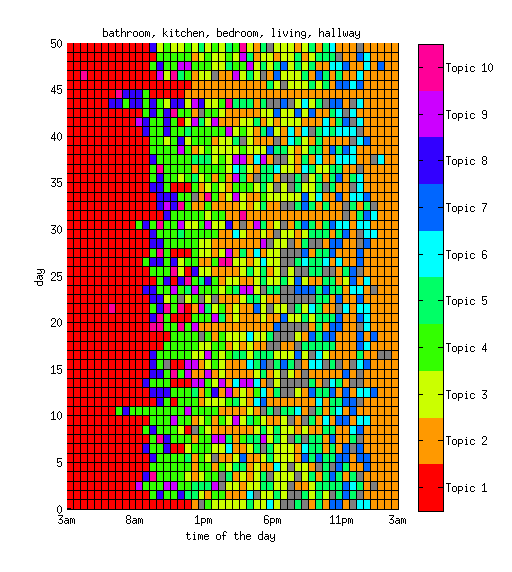
\includegraphics[width=0.45\textwidth]{Pictures/Pois/fine/DayHN1TS48k20fine.png}
  &
  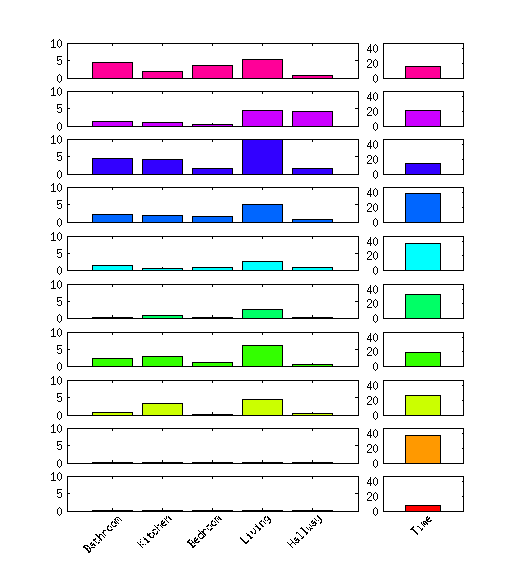
\includegraphics[width=0.45\textwidth]{Pictures/Pois/fine/TopHN1TS48k20fine.png}\\
  a) & b)
 \end{tabular}
  \caption{House number 1, 20 topics, fine grain time, LDA-Poisson}
  \label{fig:HN1Pois20fine}
\end{figure}

\begin{figure}
 \centering
 \begin{tabular}{c c}
  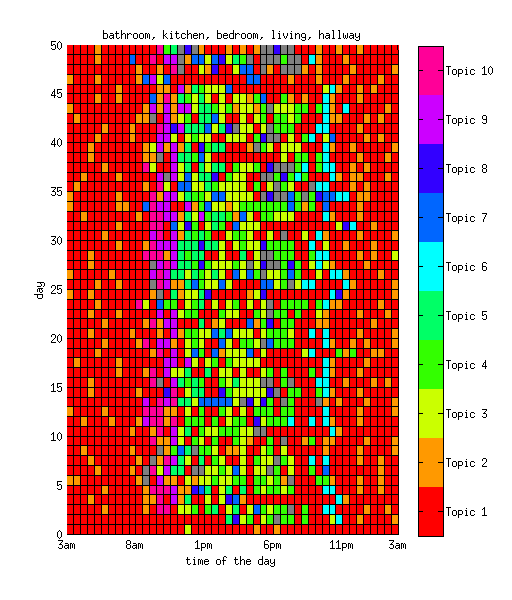
\includegraphics[width=0.45\textwidth]{Pictures/Gaus/fine/DayHN5TS48k20fine.png}
  &
  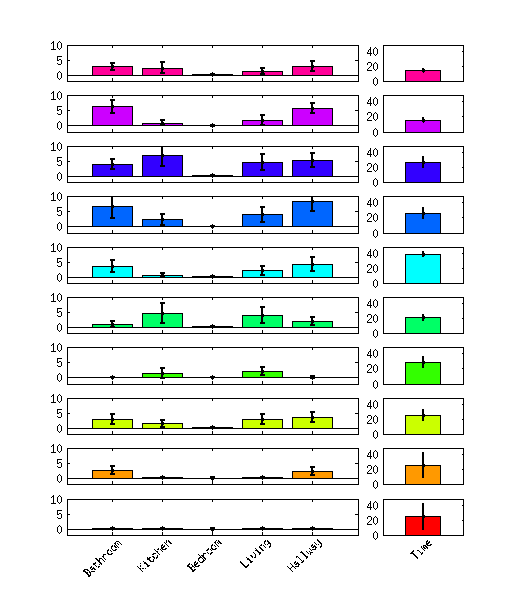
\includegraphics[width=0.45\textwidth]{Pictures/Gaus/fine/TopHN5TS48k20fine.png}\\
  a) & b)
 \end{tabular}
  \caption{House number 5, 20 topics, fine grain time, LDA-Gaussian}
  \label{fig:HN5Gaus20fine}
\end{figure}

\begin{figure}
 \centering
 \begin{tabular}{c c}
  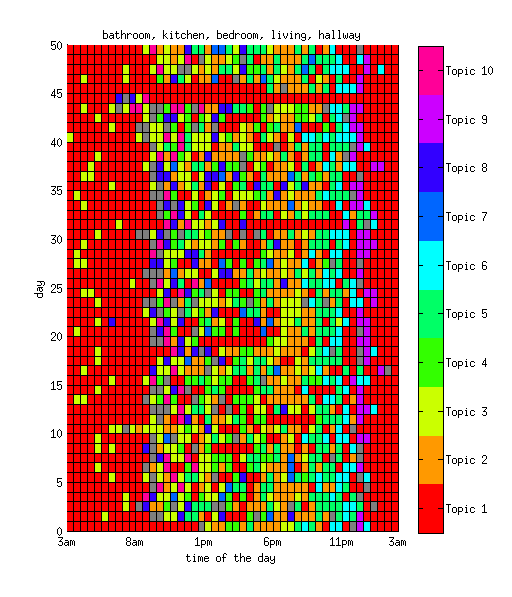
\includegraphics[width=0.45\textwidth]{Pictures/Gaus/fine/DayHN1TS48k20fine.png}
  &
  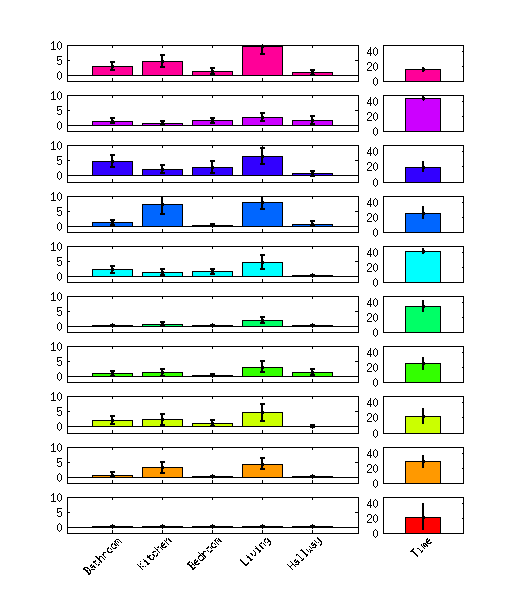
\includegraphics[width=0.45\textwidth]{Pictures/Gaus/fine/TopHN1TS48k20fine.png}\\
  a) & b)
 \end{tabular}
  \caption{House number 1, 20 topics, fine grain time, LDA-Gaussian}
  \label{fig:HN1Gaus20fine}
\end{figure}

\pagebreak

\subsection{Quantitative Results}
The log-likelihood indicates on how well the model with the estimated parameters fits the data. This can easily overfit and new data can not easily modeled with the found parameters. Therefor it is necessary to also find a high log-likelihood on a hold-out-set. The perplexity gives a good indication on how and can be calculated with
\begin{equation}
 perplexity(D_{HOS}) = exp \left\{ - \frac{\sum_{m=1}^M \log p(\textbf{o}_d ) }{M*N} \right\}
\end{equation}

A low perplexity value indicates a good result on the hold-out-set.\\

In the next experiments 10\% percent of the data is used as a hold-out set. The model is trained on the remaining 90\% with different initialization values and the perplexity is calculated on the hold-out-set with the estimated parameters. In the following it is shown what the effect is on different number of topics and different numbers of time-slices. Also the two models LDA-Gaussian and LDA-Poisson are compared with each other.

\paragraph{Different Sets of Data}
In figure \ref{fig:PerplGaus} the perplexity is shown for the 5 different data-sets gained from the 5 houses. Every run is performed ten times and the mean over these runs is taken for different number of topics $k$. Every run is initialized with 5 random days.
The data sets vary in length, but as one can see in the figure, the amount of data is not necessary of influence how well the LDA-Gaussian model can be trained. Some data sets are much more stable than others and this is probably due to the way how regular peoples behavior is.

\begin{figure}[h!]
 \centering
 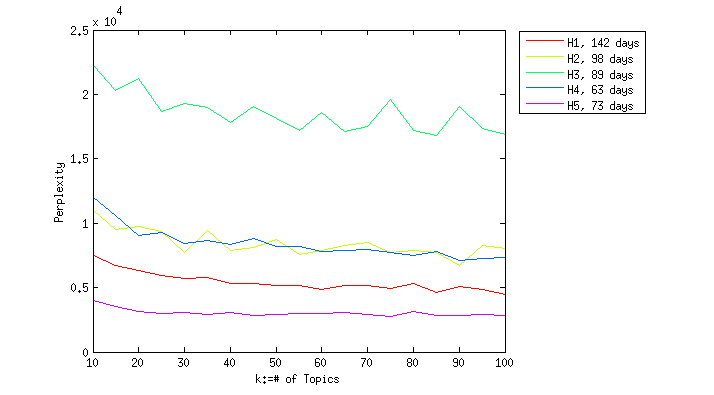
\includegraphics[width=0.7\textwidth]{Pictures/PerplGaus.png}
 \caption{Perplexity for different number of topics for 5 different House}
 \label{fig:PerplGaus}
\end{figure}

\pagebreak
\paragraph{Comparison LDA-Gaussian and LDA-Poisson}
The LDA-Poisson model is not capable to model the time dimension properly. To be able to compare both models directly with each other the time dimension is left out in the following experiments. The perplexity is calculated for the hold-out set with different amount of time-slices and the mean of 10 runs for different number of time-slices is shown in figure \ref{fig:CompareTS}. The perplexity gets better if the number of time-slices increases, but at one point the there will be no improvement. If the length of the time-slices becomes so small that only one activation is captured in an observation, the model perplexity becomes indeed very high, because a topic only contains one value. The topics are then however not very informative.\\

\begin{figure}[h!]
 \centering
  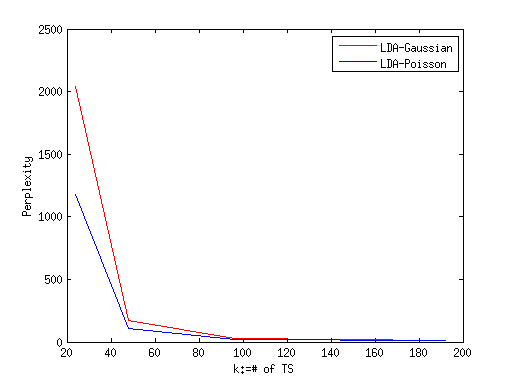
\includegraphics[width=0.7\textwidth]{Pictures/CompareTSgausPois.png}
  \caption{Perplexity for LDA-Gaussian and LDA-Poisson with different amount of time-slices}
  \label{fig:CompareTS}
\end{figure}

In figure \ref{fig:CompareK} the perplexity for both models is shown with different number of topics. The mean of 10 runs is shown and also the standard deviation is indicated with the vertical errorbar in the figure. The standard deviation increases for a higher number of topics, which is reasonable, because more topics increases the chance of more variation. If the number of topic increases the perplexity first decreases and then increases. If the number of topics is to high the model does overfit on the training data and the perplexity indeed becomes worse.\\




 \begin{figure}[h!]
  \centering
  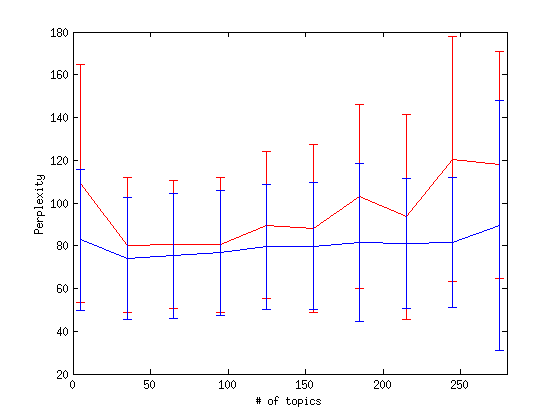
\includegraphics[width=0.7\textwidth]{Pictures/CompareCrossTops.png}
\caption{Perplexity for LDA-Gaussian and LDA-Poisson with different amount of topics}
  \label{fig:CompareK}
 \end{figure}


To creating the figures the data of house number 2 is chosen. For other data sets the outcomes looks similar and are therefore not presented. Both experiments show that the LDA-Poisson model outperforms the LDA-Gaussian model.
 
 
% \paragraph{Different length of time-slices}
% 
% In figure \ref{fig:PerplTS} we give the perplexity for different length of time-slices for the 5 Houses. We take a again the mean over 10 runs. We take for every house the same amount of days to train and test the data. We can see that with more time-slices the perplexity becomes lower for the hold-out set. For house $H2$ and $H4$ the perplexity is much better for a small amount of time-slices. The perplexities for these two houses drop much faster if the amount of time-slices increases.
% 
% \begin{figure}[h!]
%  \centering
%  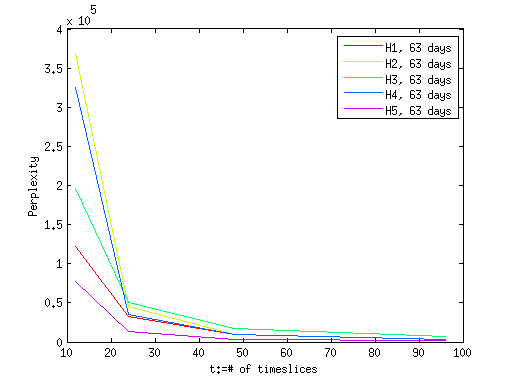
\includegraphics[width = 0.7\textwidth]{Pictures/PerplTS.png}
%  \caption{Perplexity (x-axis) for the hold-out-set for different amount of time-slices (y-axis)}
%  \label{fig:PerplTS}
% \end{figure}


% Wat wil ik nou eigenlijk aantonen en kan ik dat ook aantonen?
% Ik wil aantonen dat het nieuwe model werkt. Ik wil aantonen dat het beter werkt dan normal LDA model. 
% Het is al door meerdere mensen aangetoond dat topic modellen wel van nut zijn om behavior patronen in sensor data te vinden.
% en we kunnen dus aantonen dat onze nieuwe methode OOK werkt, want we kunnen patterns vinden. eg: een dag in de week is de persoon in de middag weg, of 's nachts moet die persoon naar het toilet

% QUALITATIVE EXPERIMENTEN
%Ik wil aantonen dat mijn model werkt en dat je wel zinnige informatie eruit kunt halen. Je kunt een semantische omschrijving van de topics geven.
%We vergelijken de nieuwe method met de BOW/k-means methode we kunnen hier ook aangeven wat de verhoudingen zijn van worden in de data en unique worden die zijn gevonden. Dit geeft ook al aan dat BOW waarschijnlijk niet werkt


%Met de gegeven data en de gekozen feature representation zijn we niet in staat om zinnige informatie uit de BOW model te halen.

% QUANTITATIVE EXPERIMENTEN


% In this section we first give some qualitative results, where the topic distribution on some days are shown. 
% Then we do something else
% Then we compare the BIC's?
% And after that we make a small test according to the feature representation.


%To test the performance of the topic models we set the variables of the features to fixed values.  In the basic LDA model we use a coarse grain value for the time. This means that the sixth dimension can have 5 different values, where the time intervals are $\{ 3am - 8am, 8am - 1pm, 1pm - 18pm, 18pm - 23pm, 23pm - 3am  \}$.